%%%%%%%%%%%%%%%%%%%%%%%%%%%%%%%%%%%%%%%%%%%%%%%%%%%%%
%			      Video Out module					%
%					-----------						%
% Author: Thibault Porteboeuf						%
%%%%%%%%%%%%%%%%%%%%%%%%%%%%%%%%%%%%%%%%%%%%%%%%%%%%%

\section{Video-Out module}

\begin{figure}[H]
\center
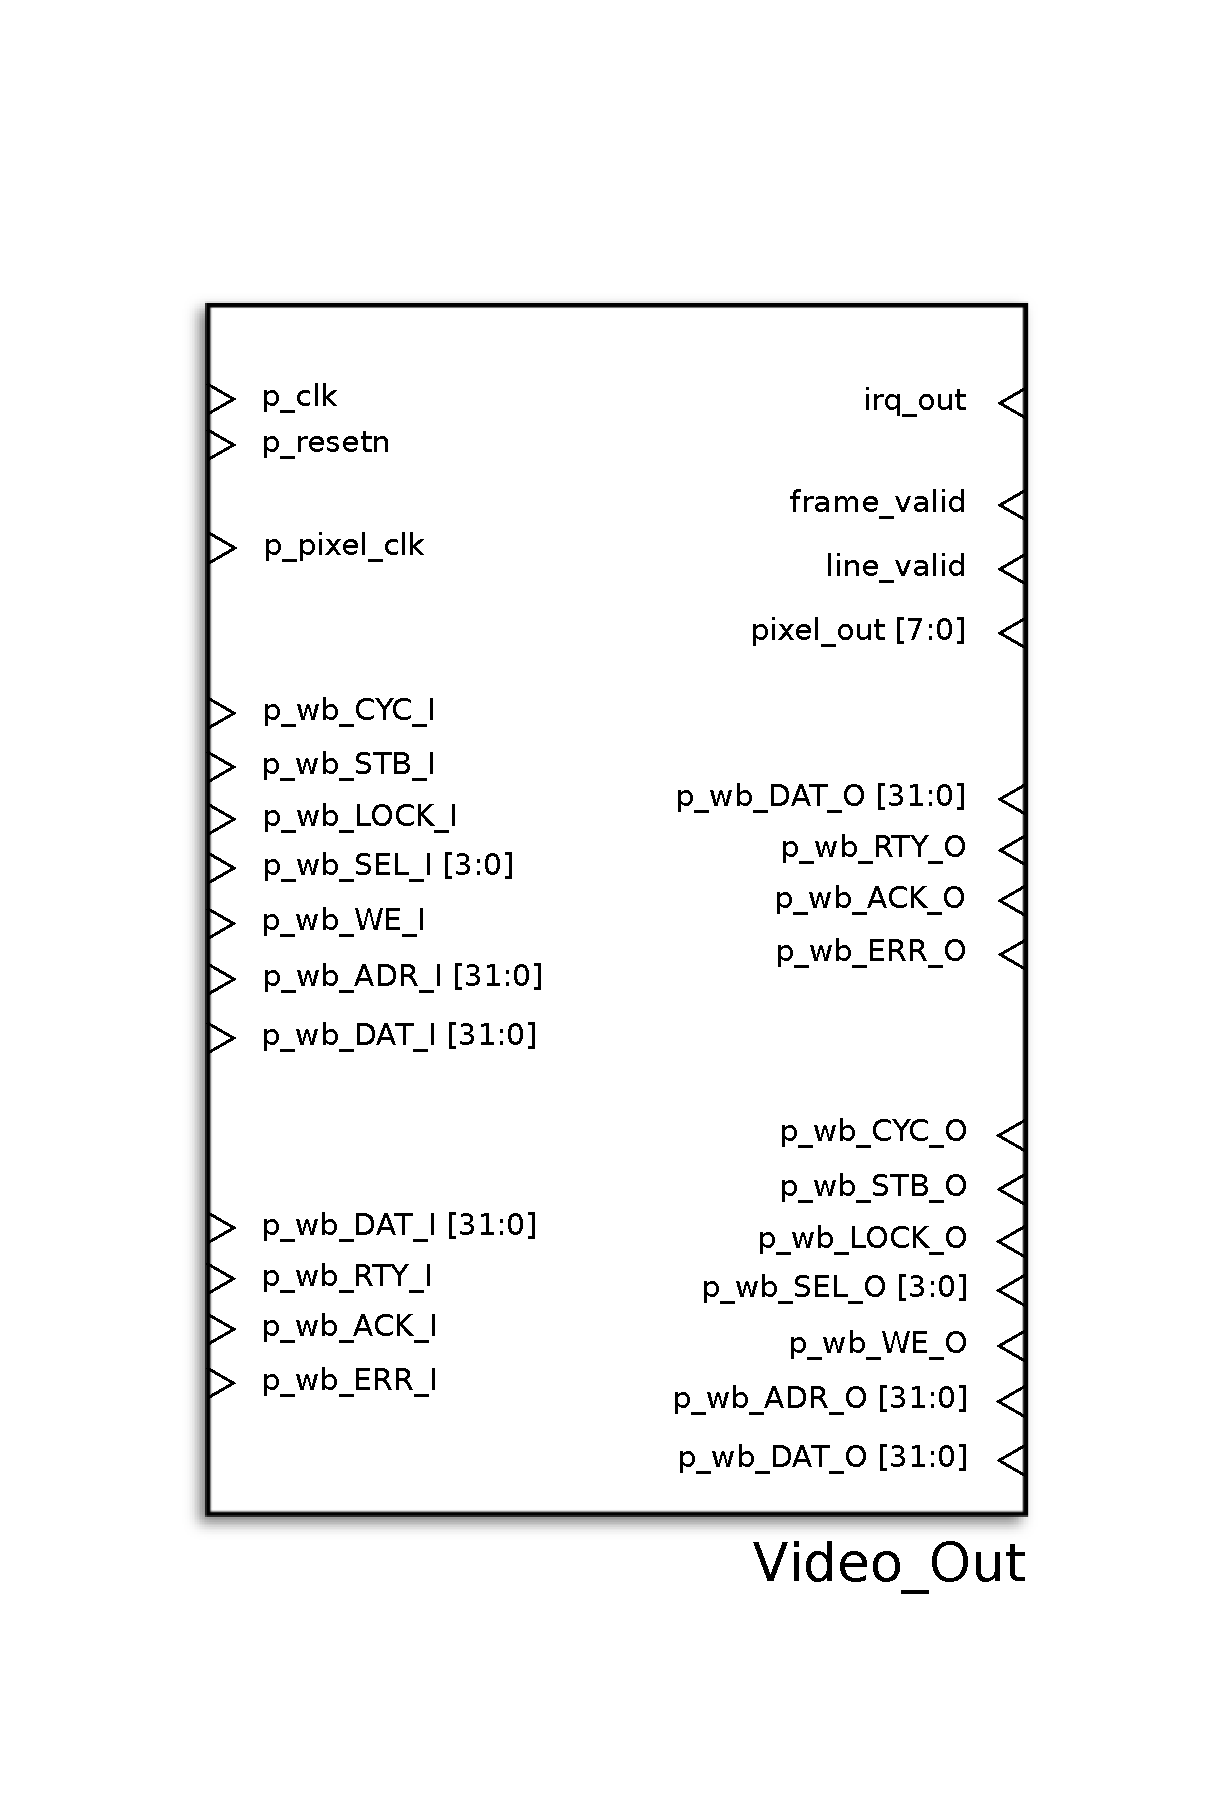
\includegraphics[width=7cm]{figs/Video_out.pdf}
\caption{VideoOut module's interface}
\label{VideoOut_interface}
\end{figure}

The Video-Out module, in design, is similar to the VideoIn module, as presented in figure \ref{VideoOut_struct}. It also has a one register slave module presented in section \ref{wb_reg_slave} and a wishbone master interface.


Video-Out is responsible to read the pixels stored on the ram and output it to the video display module.

The different ports are detailed in figure \ref{VideoOut_interface}.

The module's behavior is described in the figure \ref{VideoOut_behavior}, and is enumerated as follows:
\begin{enumerate}
\item Video-Out remains Idle until an address to read to has been written to its slave interface by LM32, as VideoIn does.
\item When this first configuration has been set, VideoOut starts pre-loading its internal buffer.
\item Video-Out starts generating the video signals and pixels while reading from the internal buffer 
\item Each time one block of buffer has been outputted to the display module, a read request is send over the wishbone bus by VideoOut's master interface, in order to retrieve more data. Care has been taken to ensure that write operations to the buffer are always one block ahead of read operations from the buffer.
\item This process continues until the end of the image, which pauses the module. It then raises an Irq in order to get the next address to read to, and starts over.
\end{enumerate}

Here again, the one register slave module is responsible for driving the Irq wire.
The state machines asks for an Irq to be raised, and the slave automatically acknowledges it once a write request has been received from the bus. In the verilog code,video in and video out instantiate this common slave module.

\vfill
\begin{figure}[h]
\center
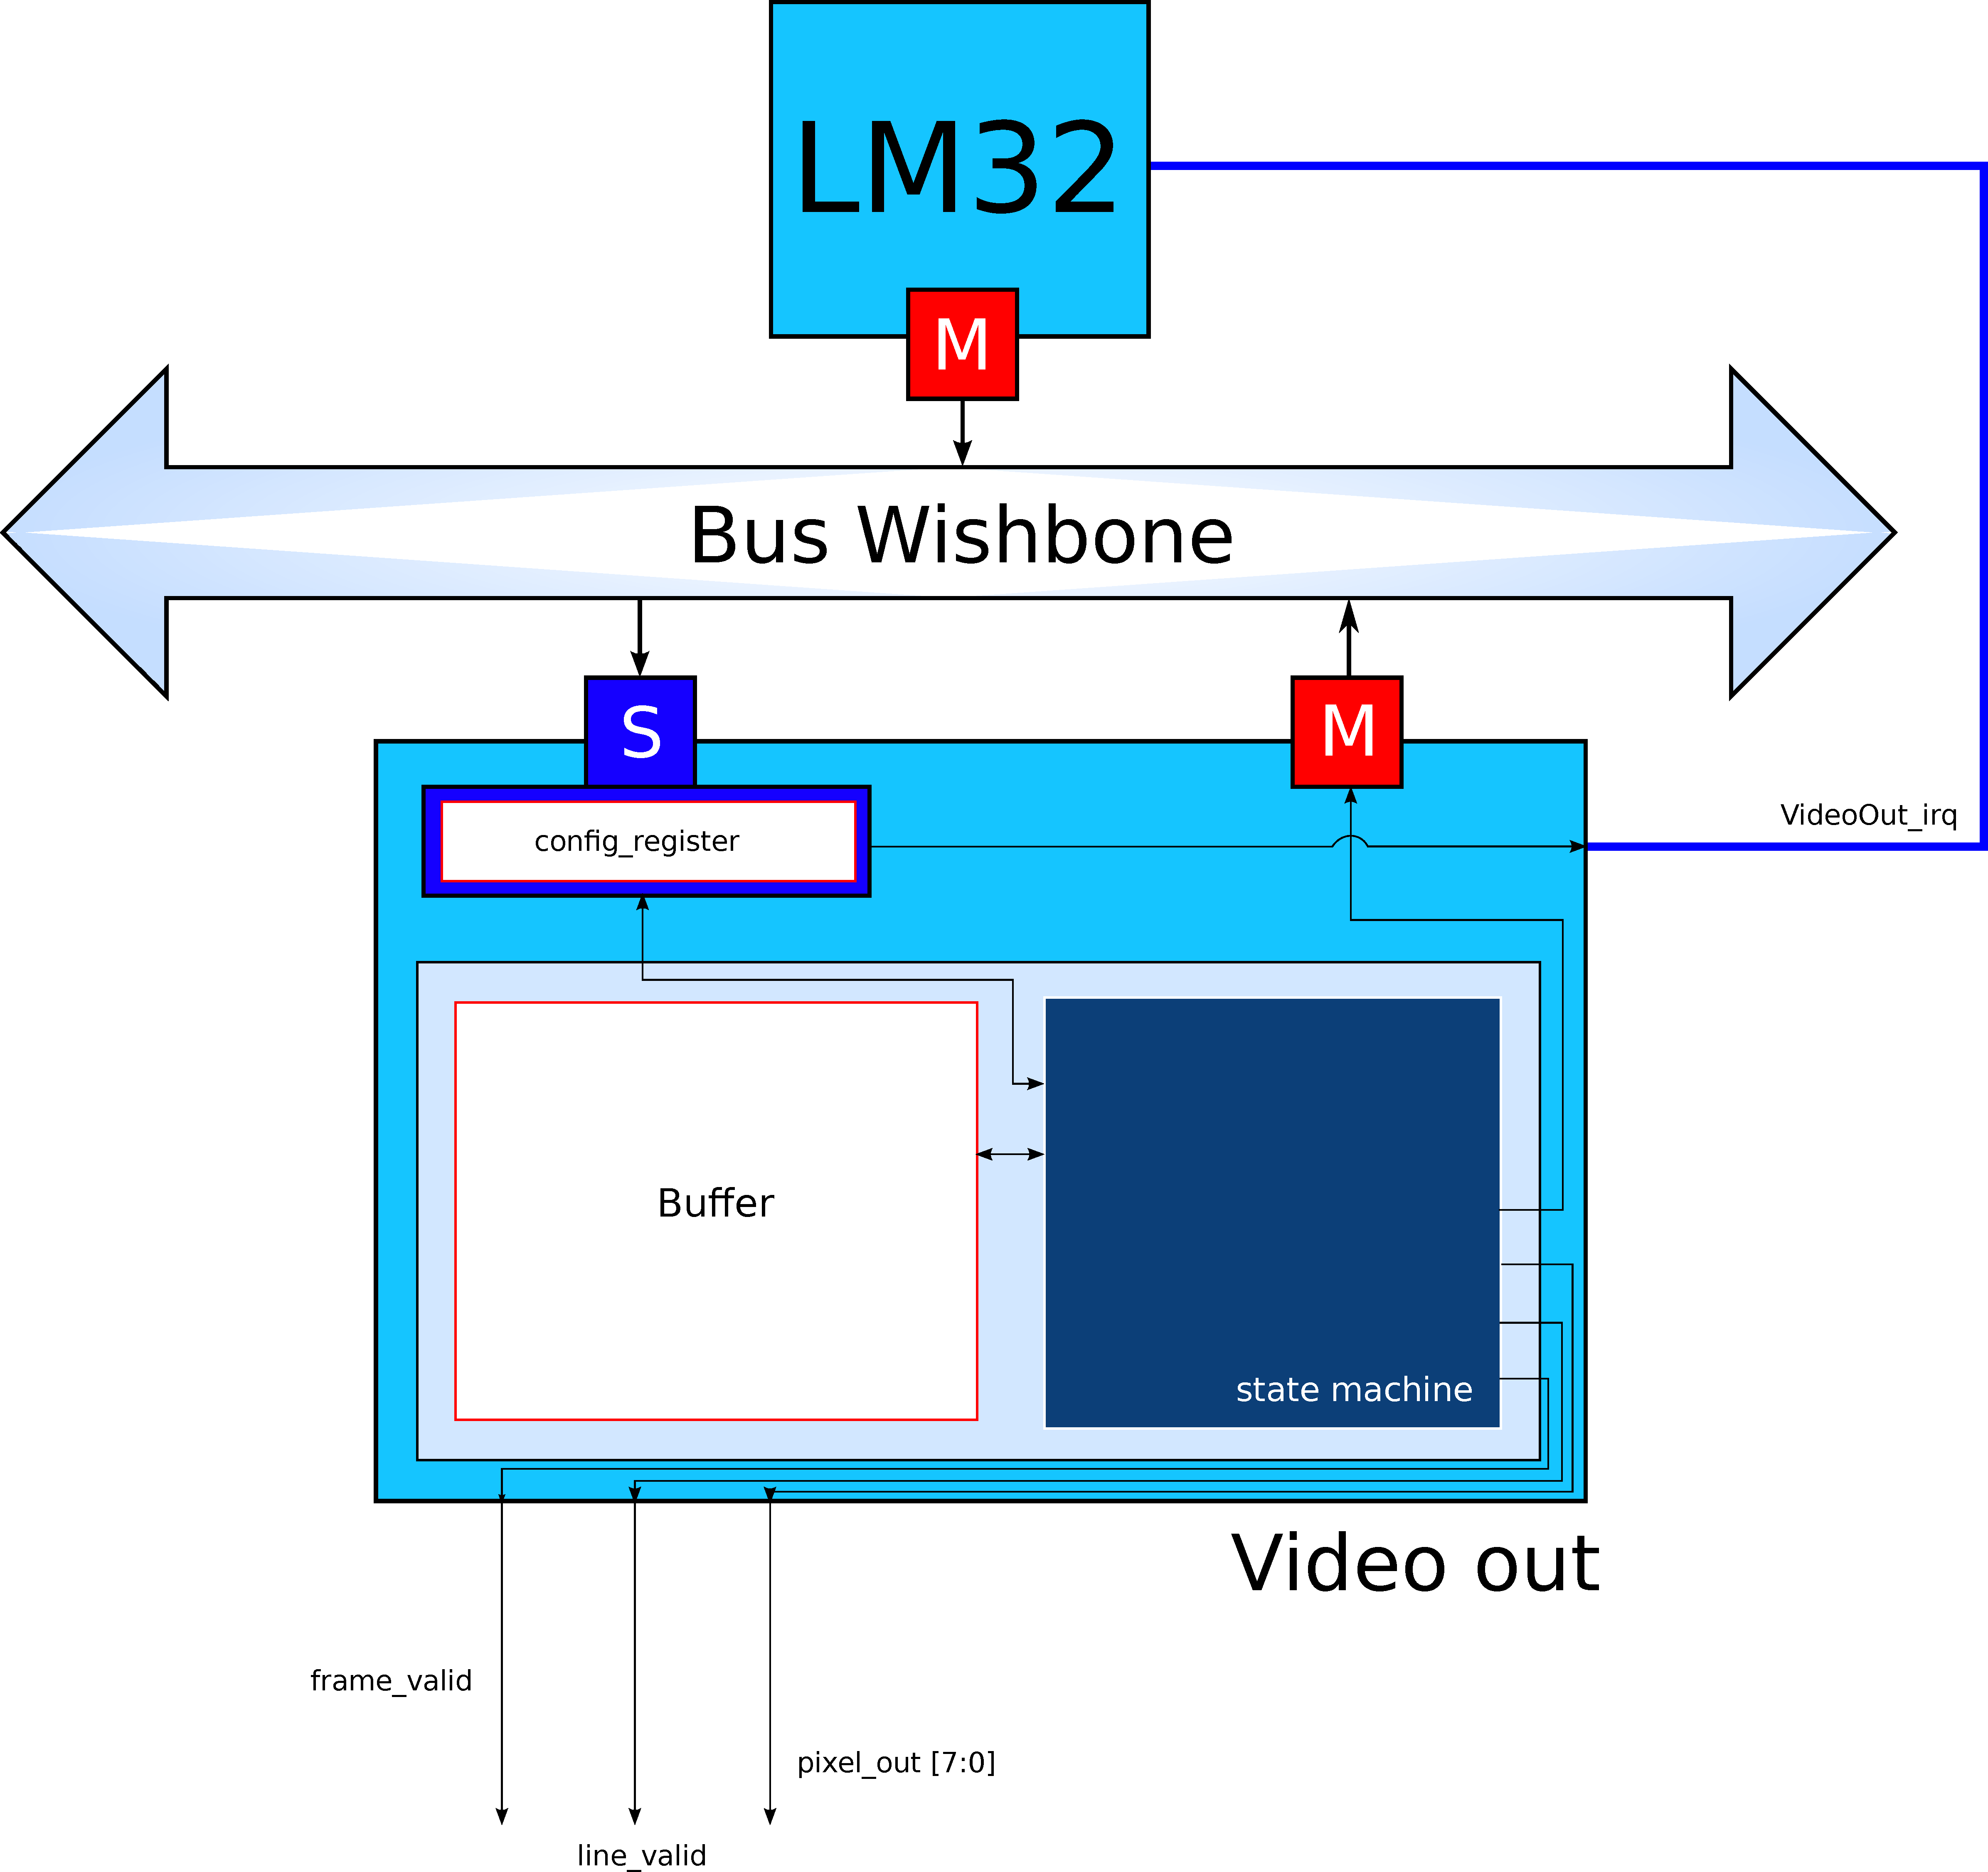
\includegraphics[width=11cm]{figs/Video_Out_blocks.pdf}
\caption{VideoOut's inner structure}
\label{VideoOut_struct}
\end{figure}
\vfill

\begin{figure}[h]
\center
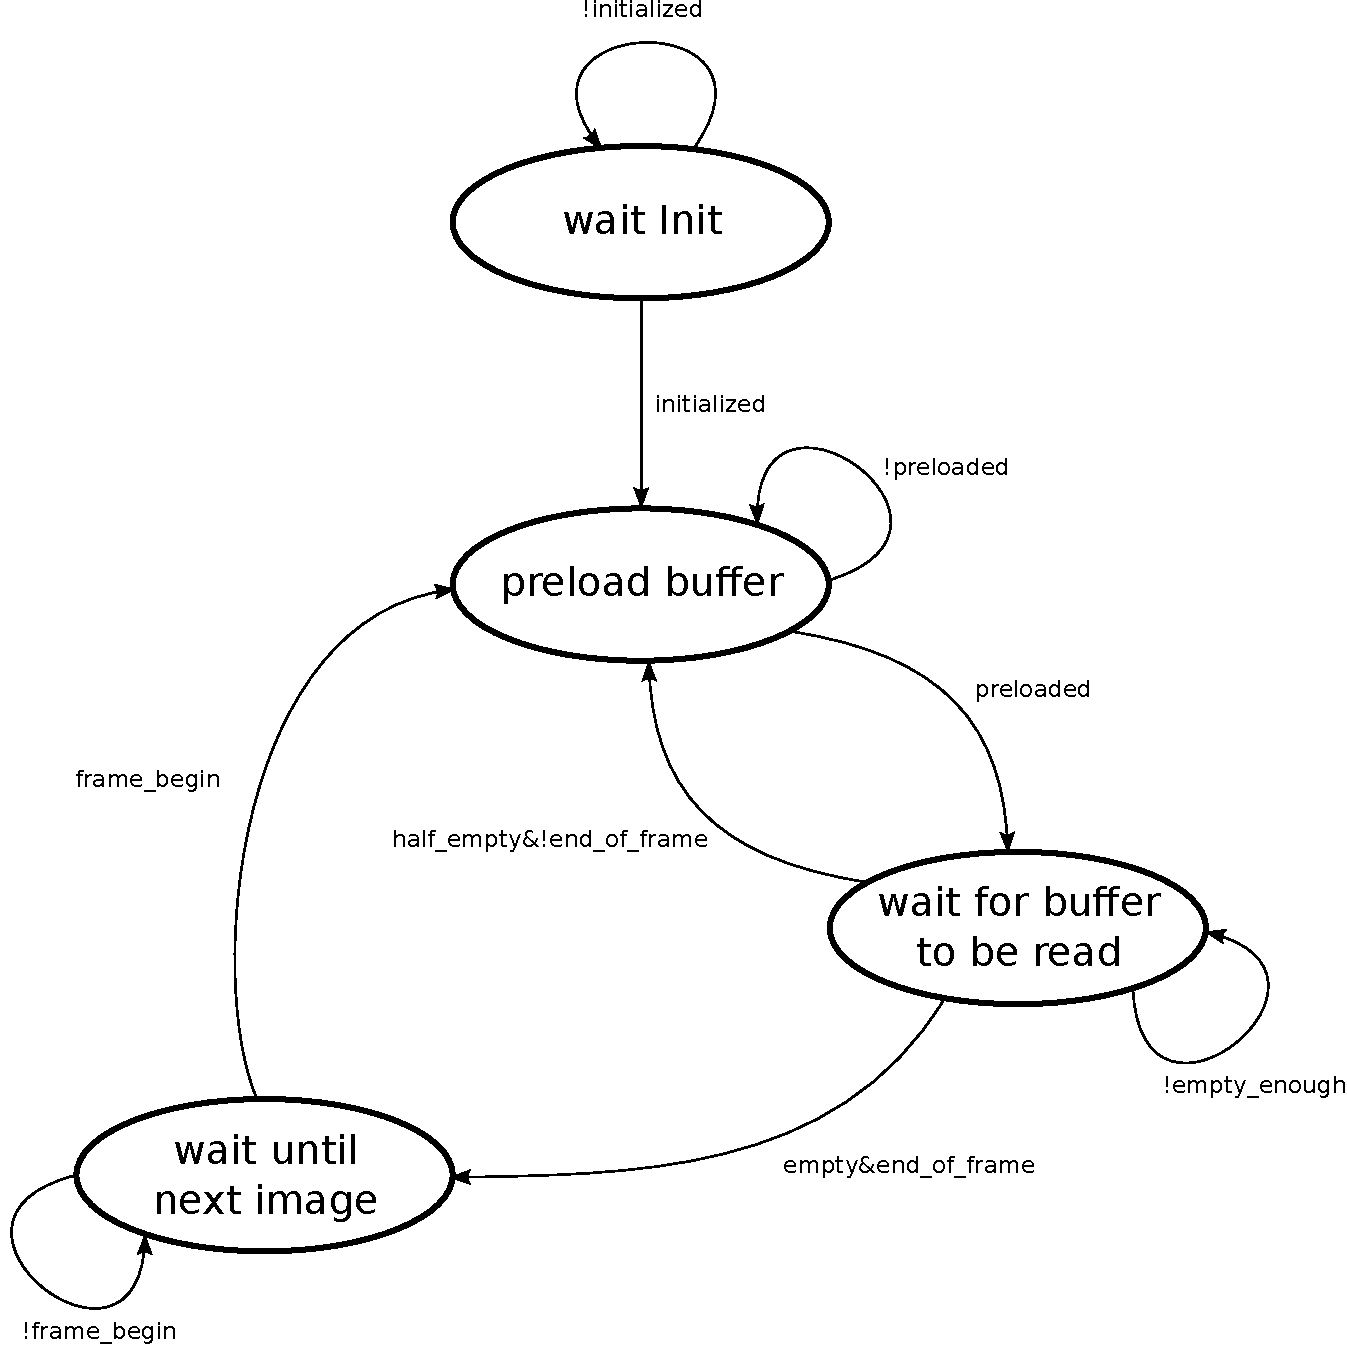
\includegraphics[width=11cm]{figs/video_out_sm.pdf}
\caption{VideoOut's behavior}
\label{VideoOut_behavior}
\end{figure}

